\documentclass[1p]{elsarticle_modified}
%\bibliographystyle{elsarticle-num}

%\usepackage[colorlinks]{hyperref}
%\usepackage{abbrmath_seonhwa} %\Abb, \Ascr, \Acal ,\Abf, \Afrak
\usepackage{amsfonts}
\usepackage{amssymb}
\usepackage{amsmath}
\usepackage{amsthm}
\usepackage{scalefnt}
\usepackage{amsbsy}
\usepackage{kotex}
\usepackage{caption}
\usepackage{subfig}
\usepackage{color}
\usepackage{graphicx}
\usepackage{xcolor} %% white, black, red, green, blue, cyan, magenta, yellow
\usepackage{float}
\usepackage{setspace}
\usepackage{hyperref}

\usepackage{tikz}
\usetikzlibrary{arrows}

\usepackage{multirow}
\usepackage{array} % fixed length table
\usepackage{hhline}

%%%%%%%%%%%%%%%%%%%%%
\makeatletter
\renewcommand*\env@matrix[1][\arraystretch]{%
	\edef\arraystretch{#1}%
	\hskip -\arraycolsep
	\let\@ifnextchar\new@ifnextchar
	\array{*\c@MaxMatrixCols c}}
\makeatother %https://tex.stackexchange.com/questions/14071/how-can-i-increase-the-line-spacing-in-a-matrix
%%%%%%%%%%%%%%%

\usepackage[normalem]{ulem}

\newcommand{\msout}[1]{\ifmmode\text{\sout{\ensuremath{#1}}}\else\sout{#1}\fi}
%SOURCE: \msout is \stkout macro in https://tex.stackexchange.com/questions/20609/strikeout-in-math-mode

\newcommand{\cancel}[1]{
	\ifmmode
	{\color{red}\msout{#1}}
	\else
	{\color{red}\sout{#1}}
	\fi
}

\newcommand{\add}[1]{
	{\color{blue}\uwave{#1}}
}

\newcommand{\replace}[2]{
	\ifmmode
	{\color{red}\msout{#1}}{\color{blue}\uwave{#2}}
	\else
	{\color{red}\sout{#1}}{\color{blue}\uwave{#2}}
	\fi
}

\newcommand{\Sol}{\mathcal{S}} %segment
\newcommand{\D}{D} %diagram
\newcommand{\A}{\mathcal{A}} %arc


%%%%%%%%%%%%%%%%%%%%%%%%%%%%%5 test

\def\sl{\operatorname{\textup{SL}}(2,\Cbb)}
\def\psl{\operatorname{\textup{PSL}}(2,\Cbb)}
\def\quan{\mkern 1mu \triangleright \mkern 1mu}

\theoremstyle{definition}
\newtheorem{thm}{Theorem}[section]
\newtheorem{prop}[thm]{Proposition}
\newtheorem{lem}[thm]{Lemma}
\newtheorem{ques}[thm]{Question}
\newtheorem{cor}[thm]{Corollary}
\newtheorem{defn}[thm]{Definition}
\newtheorem{exam}[thm]{Example}
\newtheorem{rmk}[thm]{Remark}
\newtheorem{alg}[thm]{Algorithm}

\newcommand{\I}{\sqrt{-1}}
\begin{document}

%\begin{frontmatter}
%
%\title{Boundary parabolic representations of knots up to 8 crossings}
%
%%% Group authors per affiliation:
%\author{Yunhi Cho} 
%\address{Department of Mathematics, University of Seoul, Seoul, Korea}
%\ead{yhcho@uos.ac.kr}
%
%
%\author{Seonhwa Kim} %\fnref{s_kim}}
%\address{Center for Geometry and Physics, Institute for Basic Science, Pohang, 37673, Korea}
%\ead{ryeona17@ibs.re.kr}
%
%\author{Hyuk Kim}
%\address{Department of Mathematical Sciences, Seoul National University, Seoul 08826, Korea}
%\ead{hyukkim@snu.ac.kr}
%
%\author{Seokbeom Yoon}
%\address{Department of Mathematical Sciences, Seoul National University, Seoul, 08826,  Korea}
%\ead{sbyoon15@snu.ac.kr}
%
%\begin{abstract}
%We find all boundary parabolic representation of knots up to 8 crossings.
%
%\end{abstract}
%\begin{keyword}
%    \MSC[2010] 57M25 
%\end{keyword}
%
%\end{frontmatter}

%\linenumbers
%\tableofcontents
%
\newcommand\colored[1]{\textcolor{white}{\rule[-0.35ex]{0.8em}{1.4ex}}\kern-0.8em\color{red} #1}%
%\newcommand\colored[1]{\textcolor{white}{ #1}\kern-2.17ex	\textcolor{white}{ #1}\kern-1.81ex	\textcolor{white}{ #1}\kern-2.15ex\color{red}#1	}

{\Large $\underline{10_{41}~(K10a_{35})}$}

\setlength{\tabcolsep}{10pt}
\renewcommand{\arraystretch}{1.6}
\vspace{1cm}\begin{tabular}{m{100pt}>{\centering\arraybackslash}m{274pt}}
\multirow{5}{120pt}{
	\centering
	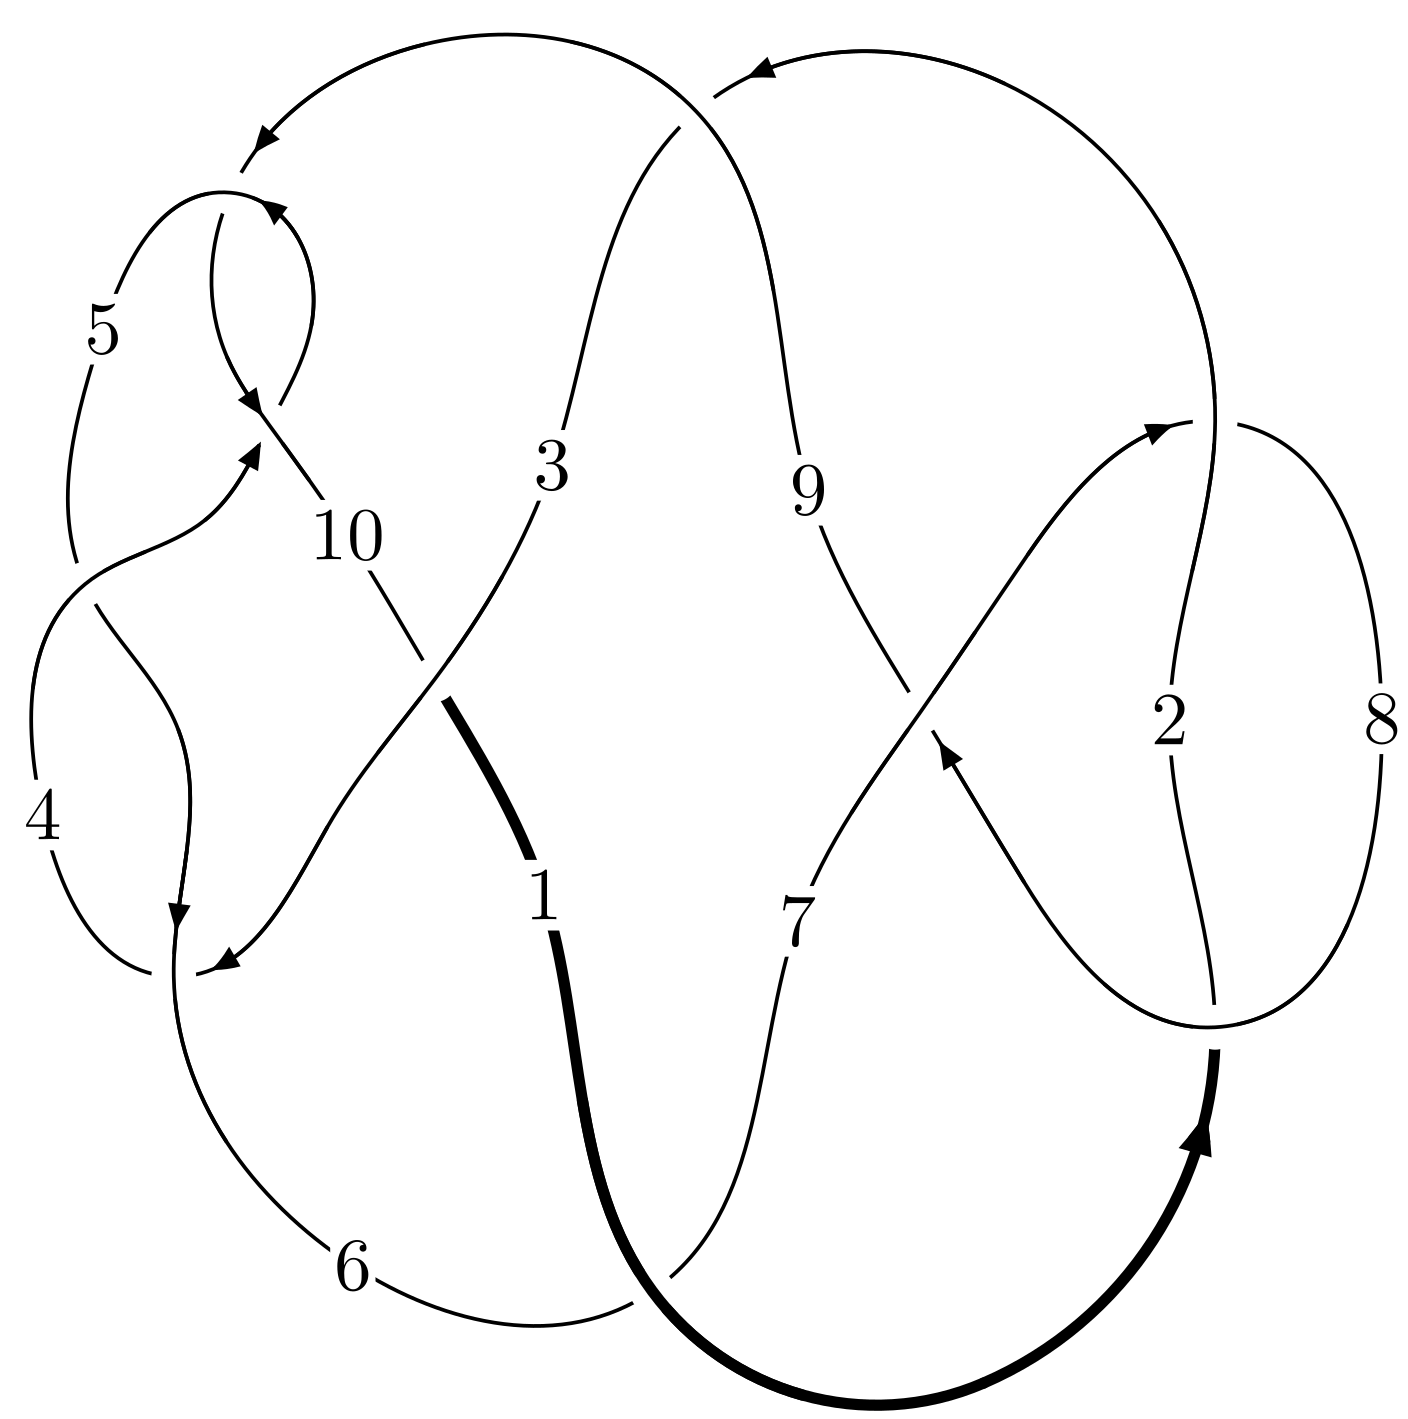
\includegraphics[width=112pt]{../../../GIT/diagram.site/Diagrams/png/125_10_41.png}\\
\ \ \ A knot diagram\footnotemark}&
\allowdisplaybreaks
\textbf{Linearized knot diagam} \\
\cline{2-2}
 &
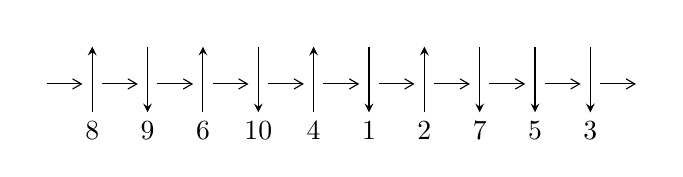
\begin{tikzpicture}[x=20pt, y=17pt]
	% nodes
	\node (C0) at (0, 0) {};
	\node (C1) at (1, 0) {};
	\node (C1U) at (1, +1) {};
	\node (C1D) at (1, -1) {8};

	\node (C2) at (2, 0) {};
	\node (C2U) at (2, +1) {};
	\node (C2D) at (2, -1) {9};

	\node (C3) at (3, 0) {};
	\node (C3U) at (3, +1) {};
	\node (C3D) at (3, -1) {6};

	\node (C4) at (4, 0) {};
	\node (C4U) at (4, +1) {};
	\node (C4D) at (4, -1) {10};

	\node (C5) at (5, 0) {};
	\node (C5U) at (5, +1) {};
	\node (C5D) at (5, -1) {4};

	\node (C6) at (6, 0) {};
	\node (C6U) at (6, +1) {};
	\node (C6D) at (6, -1) {1};

	\node (C7) at (7, 0) {};
	\node (C7U) at (7, +1) {};
	\node (C7D) at (7, -1) {2};

	\node (C8) at (8, 0) {};
	\node (C8U) at (8, +1) {};
	\node (C8D) at (8, -1) {7};

	\node (C9) at (9, 0) {};
	\node (C9U) at (9, +1) {};
	\node (C9D) at (9, -1) {5};

	\node (C10) at (10, 0) {};
	\node (C10U) at (10, +1) {};
	\node (C10D) at (10, -1) {3};
	\node (C11) at (11, 0) {};

	% arrows
	\draw[->,>={angle 60}]
	(C0) edge (C1) (C1) edge (C2) (C2) edge (C3) (C3) edge (C4) (C4) edge (C5) (C5) edge (C6) (C6) edge (C7) (C7) edge (C8) (C8) edge (C9) (C9) edge (C10) (C10) edge (C11) ;	\draw[->,>=stealth]
	(C1D) edge (C1U) (C2U) edge (C2D) (C3D) edge (C3U) (C4U) edge (C4D) (C5D) edge (C5U) (C6U) edge (C6D) (C7D) edge (C7U) (C8U) edge (C8D) (C9U) edge (C9D) (C10U) edge (C10D) ;
	\end{tikzpicture} \\
\hhline{~~} \\& 
\textbf{Solving Sequence} \\ \cline{2-2} 
 &
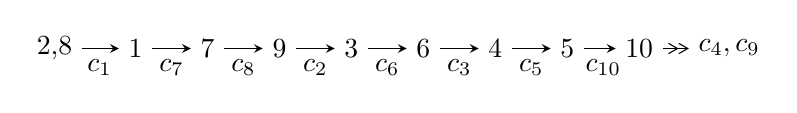
\begin{tikzpicture}[x=26pt, y=7pt]
	% node
	\node (A0) at (-1/8, 0) {2,8};
	\node (A1) at (1, 0) {1};
	\node (A2) at (2, 0) {7};
	\node (A3) at (3, 0) {9};
	\node (A4) at (4, 0) {3};
	\node (A5) at (5, 0) {6};
	\node (A6) at (6, 0) {4};
	\node (A7) at (7, 0) {5};
	\node (A8) at (8, 0) {10};
	\node (C1) at (1/2, -1) {$c_{1}$};
	\node (C2) at (3/2, -1) {$c_{7}$};
	\node (C3) at (5/2, -1) {$c_{8}$};
	\node (C4) at (7/2, -1) {$c_{2}$};
	\node (C5) at (9/2, -1) {$c_{6}$};
	\node (C6) at (11/2, -1) {$c_{3}$};
	\node (C7) at (13/2, -1) {$c_{5}$};
	\node (C8) at (15/2, -1) {$c_{10}$};
	\node (A9) at (37/4, 0) {$c_{4},c_{9}$};

	% edge
	\draw[->,>=stealth]	
	(A0) edge (A1) (A1) edge (A2) (A2) edge (A3) (A3) edge (A4) (A4) edge (A5) (A5) edge (A6) (A6) edge (A7) (A7) edge (A8) ;
	\draw[->>,>={angle 60}]	
	(A8) edge (A9);
\end{tikzpicture} \\ 

\end{tabular} \\

\footnotetext{
The image of knot diagram is generated by the software ``\textbf{Draw programme}" developed by Andrew Bartholomew(\url{http://www.layer8.co.uk/maths/draw/index.htm\#Running-draw}), where we modified some parts for our purpose(\url{https://github.com/CATsTAILs/LinksPainter}).
}\phantom \\ \newline 
\centering \textbf{Ideals for irreducible components\footnotemark of $X_{\text{par}}$} 
 
\begin{align*}
I^u_{1}&=\langle 
u^{35}+u^{34}+\cdots-2 u-1\rangle \\
\\
\end{align*}
\raggedright * 1 irreducible components of $\dim_{\mathbb{C}}=0$, with total 35 representations.\\
\footnotetext{All coefficients of polynomials are rational numbers. But the coefficients are sometimes approximated in decimal forms when there is not enough margin.}
\newpage
\renewcommand{\arraystretch}{1}
\centering \section*{I. $I^u_{1}= \langle u^{35}+u^{34}+\cdots-2 u-1 \rangle$}
\flushleft \textbf{(i) Arc colorings}\\
\begin{tabular}{m{7pt} m{180pt} m{7pt} m{180pt} }
\flushright $a_{2}=$&$\begin{pmatrix}1\\0\end{pmatrix}$ \\
\flushright $a_{8}=$&$\begin{pmatrix}0\\u\end{pmatrix}$ \\
\flushright $a_{1}=$&$\begin{pmatrix}1\\u^2\end{pmatrix}$ \\
\flushright $a_{7}=$&$\begin{pmatrix}- u\\u\end{pmatrix}$ \\
\flushright $a_{9}=$&$\begin{pmatrix}- u^3\\u^3+u\end{pmatrix}$ \\
\flushright $a_{3}=$&$\begin{pmatrix}- u^6- u^4+1\\u^6+2 u^4+u^2\end{pmatrix}$ \\
\flushright $a_{6}=$&$\begin{pmatrix}u^3\\u^5+u^3+u\end{pmatrix}$ \\
\flushright $a_{4}=$&$\begin{pmatrix}u^{14}+3 u^{12}+4 u^{10}+u^8-2 u^6-2 u^4+1\\u^{16}+4 u^{14}+8 u^{12}+8 u^{10}+4 u^8\end{pmatrix}$ \\
\flushright $a_{5}=$&$\begin{pmatrix}u^{25}+6 u^{23}+\cdots+3 u^5- u\\u^{27}+7 u^{25}+\cdots+u^3+u\end{pmatrix}$ \\
\flushright $a_{10}=$&$\begin{pmatrix}u^{14}+3 u^{12}+4 u^{10}+u^8-2 u^6-2 u^4+1\\- u^{14}-4 u^{12}-7 u^{10}-6 u^8-2 u^6+u^2\end{pmatrix}$\\&\end{tabular}
\flushleft \textbf{(ii) Obstruction class $= -1$}\\~\\
\flushleft \textbf{(iii) Cusp Shapes $= -4 u^{34}-4 u^{33}-36 u^{32}-32 u^{31}-156 u^{30}-128 u^{29}-412 u^{28}-320 u^{27}-712 u^{26}-548 u^{25}-792 u^{24}-652 u^{23}-472 u^{22}-508 u^{21}+56 u^{20}-156 u^{19}+380 u^{18}+184 u^{17}+328 u^{16}+304 u^{15}+108 u^{14}+176 u^{13}-36 u^{12}-8 u^{11}-56 u^{10}-88 u^9-44 u^8-64 u^7-16 u^6-12 u^5-4 u^3+4 u^2+8 u+2$}\\~\\
\newpage\renewcommand{\arraystretch}{1}
\flushleft \textbf{(iv) u-Polynomials at the component}\newline \\
\begin{tabular}{m{50pt}|m{274pt}}
Crossings & \hspace{64pt}u-Polynomials at each crossing \\
\hline $$\begin{aligned}c_{1},c_{7}\end{aligned}$$&$\begin{aligned}
&u^{35}- u^{34}+\cdots-2 u+1
\end{aligned}$\\
\hline $$\begin{aligned}c_{2},c_{6}\end{aligned}$$&$\begin{aligned}
&u^{35}+u^{34}+\cdots+10 u+1
\end{aligned}$\\
\hline $$\begin{aligned}c_{3},c_{5}\end{aligned}$$&$\begin{aligned}
&u^{35}-11 u^{34}+\cdots-2 u+1
\end{aligned}$\\
\hline $$\begin{aligned}c_{4},c_{9}\end{aligned}$$&$\begin{aligned}
&u^{35}+u^{34}+\cdots+2 u+1
\end{aligned}$\\
\hline $$\begin{aligned}c_{8}\end{aligned}$$&$\begin{aligned}
&u^{35}+19 u^{34}+\cdots-2 u-1
\end{aligned}$\\
\hline $$\begin{aligned}c_{10}\end{aligned}$$&$\begin{aligned}
&u^{35}-5 u^{34}+\cdots-54 u+13
\end{aligned}$\\
\hline
\end{tabular}\\~\\
\newpage\renewcommand{\arraystretch}{1}
\flushleft \textbf{(v) Riley Polynomials at the component}\newline \\
\begin{tabular}{m{50pt}|m{274pt}}
Crossings & \hspace{64pt}Riley Polynomials at each crossing \\
\hline $$\begin{aligned}c_{1},c_{7}\end{aligned}$$&$\begin{aligned}
&y^{35}+19 y^{34}+\cdots-2 y-1
\end{aligned}$\\
\hline $$\begin{aligned}c_{2},c_{6}\end{aligned}$$&$\begin{aligned}
&y^{35}-29 y^{34}+\cdots-50 y-1
\end{aligned}$\\
\hline $$\begin{aligned}c_{3},c_{5}\end{aligned}$$&$\begin{aligned}
&y^{35}+27 y^{34}+\cdots-22 y-1
\end{aligned}$\\
\hline $$\begin{aligned}c_{4},c_{9}\end{aligned}$$&$\begin{aligned}
&y^{35}+11 y^{34}+\cdots-2 y-1
\end{aligned}$\\
\hline $$\begin{aligned}c_{8}\end{aligned}$$&$\begin{aligned}
&y^{35}-5 y^{34}+\cdots+2 y-1
\end{aligned}$\\
\hline $$\begin{aligned}c_{10}\end{aligned}$$&$\begin{aligned}
&y^{35}-9 y^{34}+\cdots+966 y-169
\end{aligned}$\\
\hline
\end{tabular}\\~\\
\newpage\flushleft \textbf{(vi) Complex Volumes and Cusp Shapes}
$$\begin{array}{c|c|c}  
\text{Solutions to }I^u_{1}& \I (\text{vol} + \sqrt{-1}CS) & \text{Cusp shape}\\
 \hline 
\begin{aligned}
u &= -0.475306 + 0.917107 I\end{aligned}
 & -1.61985 - 2.07827 I & -4.18960 + 3.40333 I \\ \hline\begin{aligned}
u &= -0.475306 - 0.917107 I\end{aligned}
 & -1.61985 + 2.07827 I & -4.18960 - 3.40333 I \\ \hline\begin{aligned}
u &= \phantom{-}0.528952 + 0.892872 I\end{aligned}
 & -0.81872 + 7.33485 I & -2.03591 - 8.71425 I \\ \hline\begin{aligned}
u &= \phantom{-}0.528952 - 0.892872 I\end{aligned}
 & -0.81872 - 7.33485 I & -2.03591 + 8.71425 I \\ \hline\begin{aligned}
u &= -0.030366 + 1.049680 I\end{aligned}
 & -4.65111 - 2.79178 I & -9.43445 + 3.12849 I \\ \hline\begin{aligned}
u &= -0.030366 - 1.049680 I\end{aligned}
 & -4.65111 + 2.79178 I & -9.43445 - 3.12849 I \\ \hline\begin{aligned}
u &= \phantom{-}0.511218 + 0.765398 I\end{aligned}
 & \phantom{-}3.43859 + 2.09817 I & \phantom{-}4.61461 - 4.20156 I \\ \hline\begin{aligned}
u &= \phantom{-}0.511218 - 0.765398 I\end{aligned}
 & \phantom{-}3.43859 - 2.09817 I & \phantom{-}4.61461 + 4.20156 I \\ \hline\begin{aligned}
u &= -0.817305 + 0.125028 I\end{aligned}
 & -4.48418 + 7.52211 I & -3.62607 - 5.45189 I \\ \hline\begin{aligned}
u &= -0.817305 - 0.125028 I\end{aligned}
 & -4.48418 - 7.52211 I & -3.62607 + 5.45189 I \\ \hline\begin{aligned}
u &= \phantom{-}0.812555 + 0.099238 I\end{aligned}
 & -5.26005 - 1.67857 I & -5.17734 + 0.36674 I \\ \hline\begin{aligned}
u &= \phantom{-}0.812555 - 0.099238 I\end{aligned}
 & -5.26005 + 1.67857 I & -5.17734 - 0.36674 I \\ \hline\begin{aligned}
u &= -0.274169 + 0.754223 I\end{aligned}
 & -0.387744 - 1.218140 I & -4.43214 + 5.43737 I \\ \hline\begin{aligned}
u &= -0.274169 - 0.754223 I\end{aligned}
 & -0.387744 + 1.218140 I & -4.43214 - 5.43737 I \\ \hline\begin{aligned}
u &= \phantom{-}0.541549 + 0.582168 I\end{aligned}
 & \phantom{-}0.04226 - 3.00440 I & \phantom{-}0.20241 + 2.52989 I \\ \hline\begin{aligned}
u &= \phantom{-}0.541549 - 0.582168 I\end{aligned}
 & \phantom{-}0.04226 + 3.00440 I & \phantom{-}0.20241 - 2.52989 I \\ \hline\begin{aligned}
u &= -0.407102 + 1.144230 I\end{aligned}
 & -2.27261 - 1.14078 I & -3.06038 - 0.35223 I \\ \hline\begin{aligned}
u &= -0.407102 - 1.144230 I\end{aligned}
 & -2.27261 + 1.14078 I & -3.06038 + 0.35223 I \\ \hline\begin{aligned}
u &= -0.491471 + 1.162520 I\end{aligned}
 & -1.65334 - 7.02473 I & -1.60158 + 6.93954 I \\ \hline\begin{aligned}
u &= -0.491471 - 1.162520 I\end{aligned}
 & -1.65334 + 7.02473 I & -1.60158 - 6.93954 I \\ \hline\begin{aligned}
u &= \phantom{-}0.453184 + 1.179210 I\end{aligned}
 & -5.12537 + 4.24996 I & -8.86458 - 3.77353 I \\ \hline\begin{aligned}
u &= \phantom{-}0.453184 - 1.179210 I\end{aligned}
 & -5.12537 - 4.24996 I & -8.86458 + 3.77353 I \\ \hline\begin{aligned}
u &= -0.386425 + 1.221160 I\end{aligned}
 & -8.54235 + 3.42594 I & -8.10972 - 2.22817 I \\ \hline\begin{aligned}
u &= -0.386425 - 1.221160 I\end{aligned}
 & -8.54235 - 3.42594 I & -8.10972 + 2.22817 I \\ \hline\begin{aligned}
u &= -0.703066 + 0.147767 I\end{aligned}
 & \phantom{-}1.26318 + 2.51214 I & \phantom{-}2.03969 - 3.87852 I \\ \hline\begin{aligned}
u &= -0.703066 - 0.147767 I\end{aligned}
 & \phantom{-}1.26318 - 2.51214 I & \phantom{-}2.03969 + 3.87852 I \\ \hline\begin{aligned}
u &= \phantom{-}0.402291 + 1.220240 I\end{aligned}
 & -9.20933 + 2.50696 I & -9.26110 - 2.94934 I \\ \hline\begin{aligned}
u &= \phantom{-}0.402291 - 1.220240 I\end{aligned}
 & -9.20933 - 2.50696 I & -9.26110 + 2.94934 I \\ \hline\begin{aligned}
u &= \phantom{-}0.714433\phantom{ +0.000000I}\end{aligned}
 & -1.80251\phantom{ +0.000000I} & -5.77680\phantom{ +0.000000I} \\ \hline\begin{aligned}
u &= \phantom{-}0.498606 + 1.204550 I\end{aligned}
 & -8.52390 + 6.46046 I & -8.19651 - 3.55460 I\\
 \hline 
 \end{array}$$\newpage$$\begin{array}{c|c|c}  
\text{Solutions to }I^u_{1}& \I (\text{vol} + \sqrt{-1}CS) & \text{Cusp shape}\\
 \hline 
\begin{aligned}
u &= \phantom{-}0.498606 - 1.204550 I\end{aligned}
 & -8.52390 - 6.46046 I & -8.19651 + 3.55460 I \\ \hline\begin{aligned}
u &= -0.509525 + 1.201690 I\end{aligned}
 & -7.6692 - 12.3766 I & -6.59656 + 8.49008 I \\ \hline\begin{aligned}
u &= -0.509525 - 1.201690 I\end{aligned}
 & -7.6692 + 12.3766 I & -6.59656 - 8.49008 I \\ \hline\begin{aligned}
u &= -0.510838 + 0.446804 I\end{aligned}
 & -0.37526 - 1.90476 I & -0.38240 + 3.26312 I \\ \hline\begin{aligned}
u &= -0.510838 - 0.446804 I\end{aligned}
 & -0.37526 + 1.90476 I & -0.38240 - 3.26312 I\\
 \hline 
 \end{array}$$\newpage
\newpage\renewcommand{\arraystretch}{1}
\centering \section*{ II. u-Polynomials}
\begin{tabular}{m{50pt}|m{274pt}}
Crossings & \hspace{64pt}u-Polynomials at each crossing \\
\hline $$\begin{aligned}c_{1},c_{7}\end{aligned}$$&$\begin{aligned}
&u^{35}- u^{34}+\cdots-2 u+1
\end{aligned}$\\
\hline $$\begin{aligned}c_{2},c_{6}\end{aligned}$$&$\begin{aligned}
&u^{35}+u^{34}+\cdots+10 u+1
\end{aligned}$\\
\hline $$\begin{aligned}c_{3},c_{5}\end{aligned}$$&$\begin{aligned}
&u^{35}-11 u^{34}+\cdots-2 u+1
\end{aligned}$\\
\hline $$\begin{aligned}c_{4},c_{9}\end{aligned}$$&$\begin{aligned}
&u^{35}+u^{34}+\cdots+2 u+1
\end{aligned}$\\
\hline $$\begin{aligned}c_{8}\end{aligned}$$&$\begin{aligned}
&u^{35}+19 u^{34}+\cdots-2 u-1
\end{aligned}$\\
\hline $$\begin{aligned}c_{10}\end{aligned}$$&$\begin{aligned}
&u^{35}-5 u^{34}+\cdots-54 u+13
\end{aligned}$\\
\hline
\end{tabular}\newpage\renewcommand{\arraystretch}{1}
\centering \section*{ III. Riley Polynomials}
\begin{tabular}{m{50pt}|m{274pt}}
Crossings & \hspace{64pt}Riley Polynomials at each crossing \\
\hline $$\begin{aligned}c_{1},c_{7}\end{aligned}$$&$\begin{aligned}
&y^{35}+19 y^{34}+\cdots-2 y-1
\end{aligned}$\\
\hline $$\begin{aligned}c_{2},c_{6}\end{aligned}$$&$\begin{aligned}
&y^{35}-29 y^{34}+\cdots-50 y-1
\end{aligned}$\\
\hline $$\begin{aligned}c_{3},c_{5}\end{aligned}$$&$\begin{aligned}
&y^{35}+27 y^{34}+\cdots-22 y-1
\end{aligned}$\\
\hline $$\begin{aligned}c_{4},c_{9}\end{aligned}$$&$\begin{aligned}
&y^{35}+11 y^{34}+\cdots-2 y-1
\end{aligned}$\\
\hline $$\begin{aligned}c_{8}\end{aligned}$$&$\begin{aligned}
&y^{35}-5 y^{34}+\cdots+2 y-1
\end{aligned}$\\
\hline $$\begin{aligned}c_{10}\end{aligned}$$&$\begin{aligned}
&y^{35}-9 y^{34}+\cdots+966 y-169
\end{aligned}$\\
\hline
\end{tabular}
\vskip 2pc
\end{document}